\chapter{CAM3 and AM2 clouds in present-day climate}
\label{cmip3amip}
\section{Introduction}
This chapter presents an evaluation of the relative performance of two climate models in simulating statistics of cloud properties in present-day climate. The GFDL AM2 and NCAR CAM3 are chosen for this two-model inter-comparison. The CFMIP Observation Simulator Package is used to facilitate comparisons between modeled and observed cloud statistics, and to provide a common framework for comparison of the relative performance of the two models.

The two models used in this chapter were part of the CMIP3 and were referenced in the IPCC Fourth Assessment Report. Development of each of these models has since continued, and new versions are available. However, a critical evaluation of the past generation of models provides a framework for assessing future model changes and determining to what extent development has improved model climate simulations.

Additionally, evaluation of the past generation of models provides a baseline for assessing the changes in simulated climate in climate change experiments. This is done in Chapter \ref{cmip3hot}. The results presented in this chapter provide a framework for understanding the changes in the simulated climates that occur in the climate change experiments.

It is shown here that simulations with CAM3 and AM2 tend to underestimate total and especially low-topped cloud amount compared with observations from ISCCP, MISR, and MODIS. The effect of the underestimation of cloudiness on the top of atmosphere radiative fluxes is at least partly compensated for by an overestimation of optically intermediate and optically thick cloud amount. Similar results were found by \cite{zhang_et_al_2005}, who used output from the ISCCP simulator to quantify biases between models and observations from ISCCP and CERES. The intercomparison included the GFDL AM2, and the NCAR CAM2 (an earlier version of the NCAR model used in this study). The addition of MISR and MODIS observations and simulators in this study increases the robustness of many of the conclusions of \cite{zhang_et_al_2005}.

Different geographical regions on the globe are characterized by different dominant cloud types. Because different cloud types have different radiative impacts \citep{dhuria_and_kyle_1990,hartmann_and_michelsen_1993}, and because climate models often employ different physics parameterizations for different conditions or regions \citep[e.g.,][]{cam3_description}, it is important to separately and critically evaluate model simulation of clouds in different regions or regimes. This will be done here for a selection of regions in the tropics and subtropics.

\section{Model and experiment set-up}
The results shown in this chapter are from ``AMIP''-style runs, in which the models are forced with observed monthly-mean sea-surface temperature data. Both CAM3 and AM2 simulations were performed for the model time period 1990-2000. Ideally, these runs would be performed for the same period for which observational data is available from the remote sensing instruments used in this study. Although this period does overlap with the ISCCP observational record, MISR data is only available back to March of 2000, and MODIS data to 2002. Unfortunately, the needed input data were not available at the time to run CAM3 and AM2 beyond 2000 (input data for AM2 ends in 1999 and climatological mean sea-surface temperatures were used to finish the last year of the AM2 run). Nonetheless, Figure \ref{cldtot_obs_taylor} suggests that observed cloud fields should not be drastically different over these differing periods, and it is shown here that the modeled cloud properties differ substantially from the observations so as to make the small differences expected between these two periods unimportant to the overall conclusions.

\section{Results}
\subsection{Global evaluation of clouds and radiation in CAM3 and AM2 AMIP simulations}
Clouds are of primary importance in climate models due to the impact they have on the top of atmosphere radiative balance. This can be quantified by calculating cloud radiative effect (often misleadingly referred to as ``cloud radiative forcing''), defined as the difference in the top of atmosphere radiation balance between the all-sky and clear-sky atmosphere \citep{ramanathan_et_al_1989}. Figures \ref{swcrebiases_cmip3amip_map} and \ref{lwcrebiases_cmip3amip_map} show the differences in shortwave and longwave components of the cloud radiative effect between CAM3 and AM2 AMIP simulations and observations from CERES-EBAF (note that the longwave cloud radiative effect is independent of the simulator package, and uses the raw model-diagnosed cloud fraction to distinguish all-sky from clear-sky). Because the shortwave cloud radiative effect is negative due to clouds being highly reflective in the shortwave, negative bias values indicate an enhanced shortwave cooling effect of clouds. The longwave cloud radiative effect is positive, so positive bias values indicate an enhanced longwave heating effect of clouds. The values of the global mean bias in the two models compared to the observations are small relative to the large regional biases, indicating that regional biases in the representation of clouds in the models compensate to achieve a reasonable estimation of the radiative impact of clouds in the global mean sense. Figure \ref{cre_cmip3amip_taylor} clearly demonstrates this in a statistical sense. The magnitude of the shortwave and longwave cloud radiative effect in both models closely matches that in the observations (indicated by small relative biases), although the correlation in these fields in space and time is unimpressive. The AM2 simulation of shortwave and longwave cloud radiative effect more closely matches the observations than does CAM3, with higher space-time correlation and variance ratios closer to unity for both the shortwave and the longwave, and smaller biases in the shortwave. 

The sign of the global annual mean biases in longwave cloud radiative effect differs between the two models, with a positive bias in the CAM3 simulation and a negative bias in the AM2 simulation. The net cloud radiative effect is similar between the two models because the positive bias in longwave cloud radiative effect in the CAM3 simulation partially compensates the larger negative bias in the shortwave cloud radiative effect seen in the CAM3 simulation. This compensation between longwave and shortwave cloud radiative effect is evident in the regional biases as well; regions with large negative biases in shortwave cloud radiative effect tend to show large positive biases in longwave cloud radiative effect, and vice versa.

\begin{figure}
    \centering
    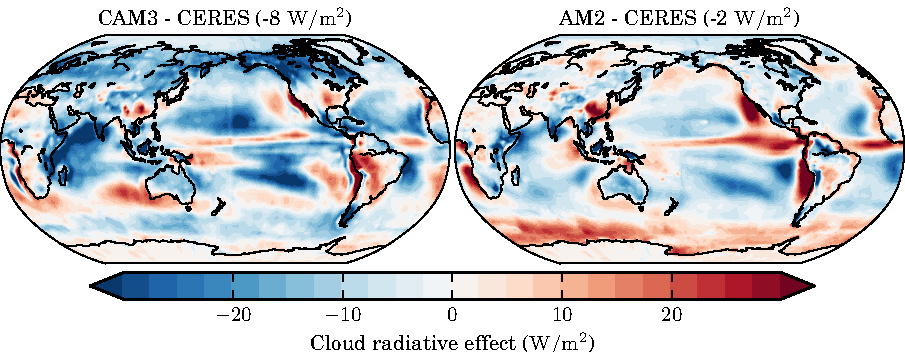
\includegraphics{../graphics/swcrebiases_cmip3amip_map.pdf}
    \caption[Biases in shortwave cloud radiative effect in CAM3 and AM2 AMIP simulations compared with observations from CERES-EBAF.]{Biases in shortwave cloud radiative effect in CAM3 and AM2 AMIP simulations compared with observations from CERES-EBAF. Values in the titles of the individual plots indicate the area-weighted global mean bias.}
    \label{swcrebiases_cmip3amip_map}
\end{figure}

\begin{figure}
    \centering
    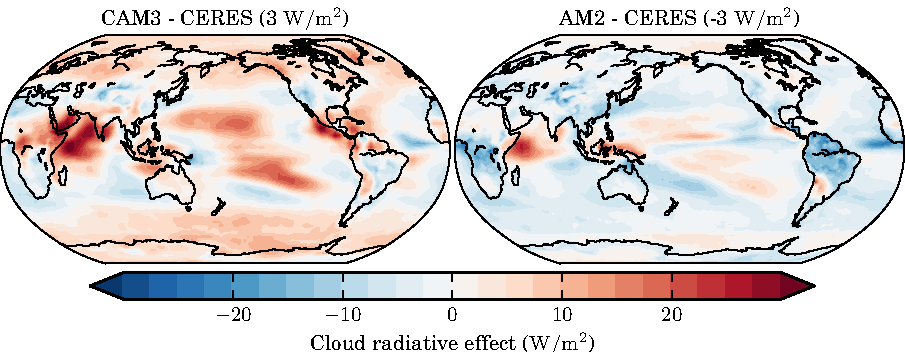
\includegraphics{../graphics/lwcrebiases_cmip3amip_map.pdf}
    \caption[Biases in longwave cloud radiative effect in CAM3 and AM2 AMIP simulations compared with observations from CERES-EBAF.]{Biases in longwave cloud radiative effect in CAM3 and AM2 AMIP simulations compared with observations from CERES-EBAF. Values in the titles of the individual plots indicate the area-weighted global mean bias.}
    \label{lwcrebiases_cmip3amip_map}
\end{figure}

\begin{figure}
    \centering
    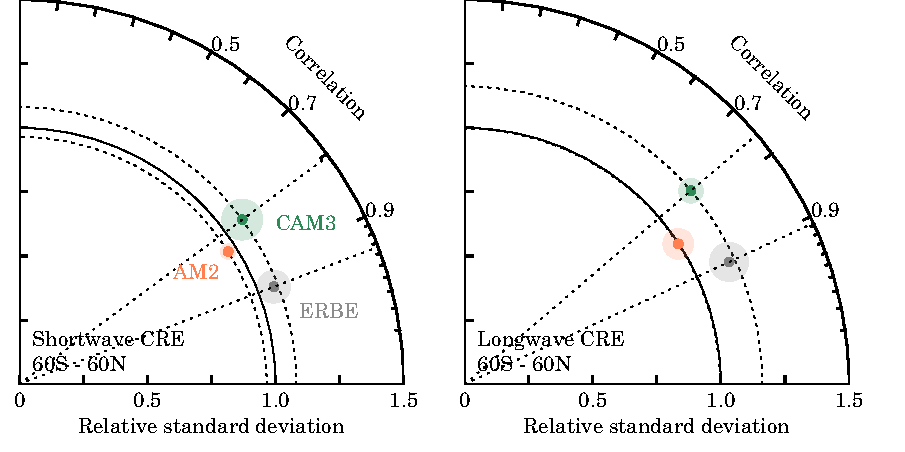
\includegraphics{../graphics/cre_cmip3amip_taylor.pdf}
    \caption[Taylor diagrams comparing shortwave and longwave cloud radiative effect from CAM3 and AM2 AMIP simulations with observations from CERES-EBAF.]{Taylor diagrams comparing shortwave and longwave cloud radiative effect from CAM3 and AM2 AMIP simulations with observations from CERES-EBAF. Shortwave and longwave cloud radiative effect from the Earth Radiative Budget Experiment (ERBE) \citep{harrison_et_al_1990} are compared against the CERES-EBAF dataset as well.}
    \label{cre_cmip3amip_taylor}
\end{figure}
    
Cloud radiative effect is regulated in part by the amount of cloud. Figure \ref{cldtypes_cmip3amip_bar} shows that both the CAM3 and AM2 simulations underestimate both the total and low-topped cloud amounts when compared with ISCCP, MISR, or MODIS. Note that this figure shows MODIS cloud amounts taken before clear-sky restoral, which are not subject to the optical thickness threshold cut-off as the ISCCP and MISR cloud amounts are. The shortwave cooling effect dominates the cloud radiative effect for low-topped clouds, so the underestimation of low-topped cloud would cause an underestimation of the shortwave cooling effect of clouds in the absence of other biases in the cloud properties. The fact that the shortwave cooling effect of clouds can be overestimated by both models while total and low-topped cloud amount is grossly underestimated is reconciled by Figure \ref{tau_cmip3amip}, which shows that, while total cloud amount is underestimated, the distribution of cloud with optical thickness is biased toward higher values. The bias toward higher optical thickness means that the clouds are brighter and hence reflect more shortwave radiation back to space, leading to an enhanced shortwave cooling effect.
\begin{figure}
    \centering
    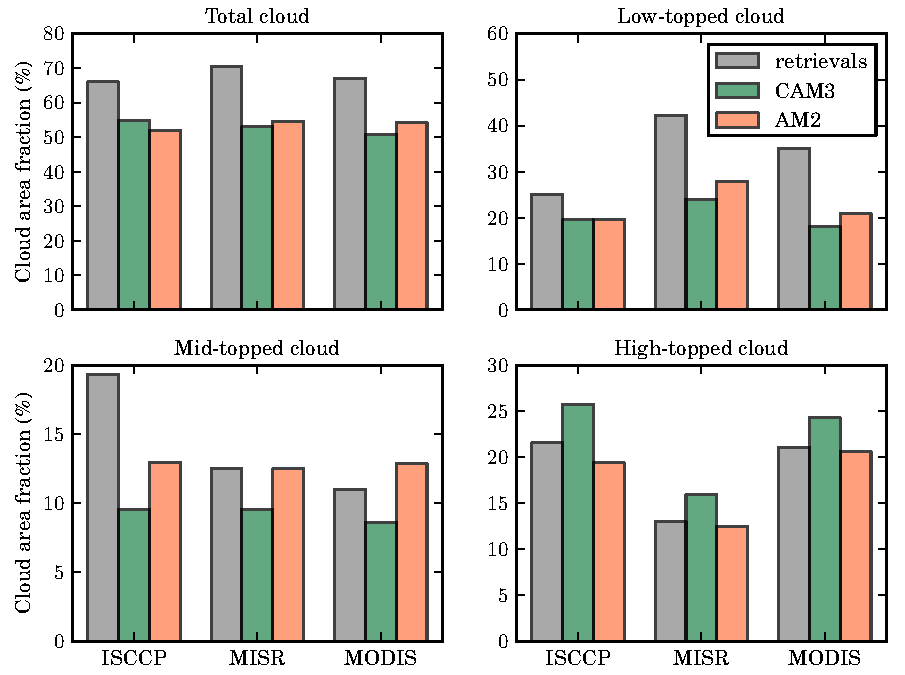
\includegraphics{../graphics/cldtypes_cmip3amip_bar.pdf} 
    \caption[Total, low-topped, mid-topped, and high-topped cloud amounts from ISCCP, MISR, and MODIS and the corresponding simulator diagnostics from CAM3 and AM2 AMIP simulations]{Total, low-topped, mid-topped, and high-topped cloud amounts from ISCCP, MISR, and MODIS and the corresponding simulator diagnostics from CAM3 and AM2 AMIP simulations. MODIS cloud amounts are taken before clear-sky restoral.}
    \label{cldtypes_cmip3amip_bar}
\end{figure}

\begin{figure}
    \centering
    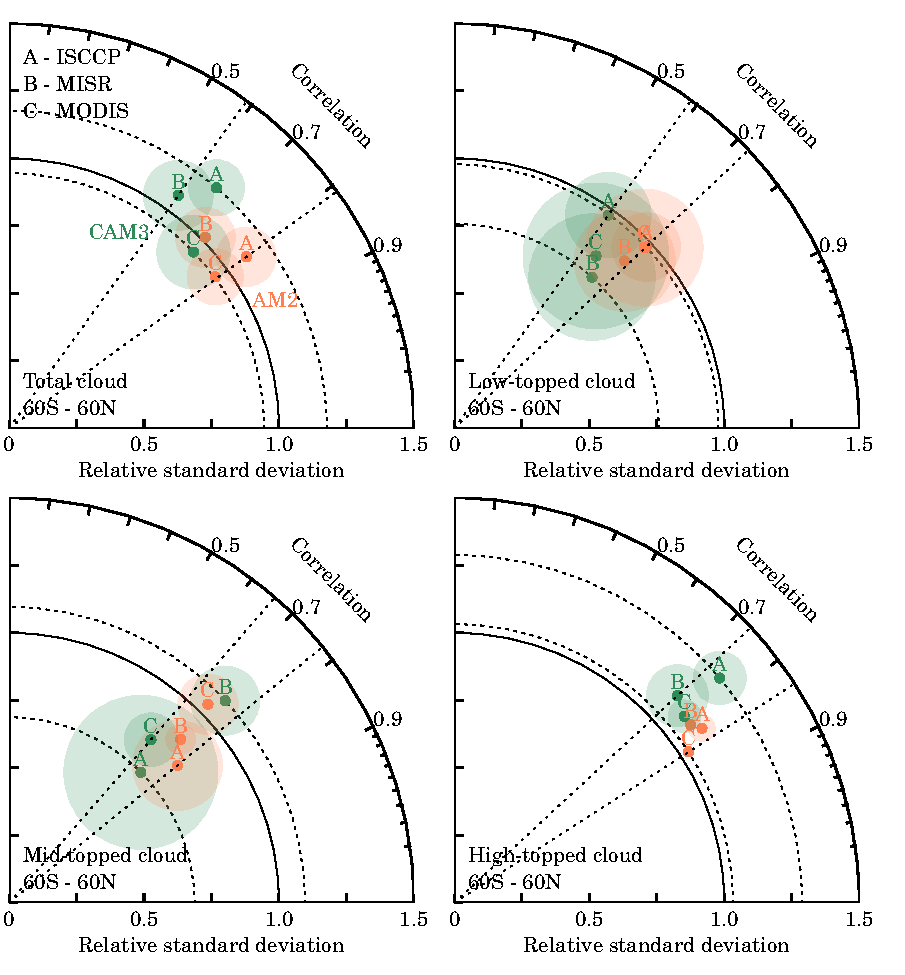
\includegraphics{../graphics/cldtypes_cmip3amip_taylor.pdf} 
    \caption[Taylor diagrams comparing total, low-topped, mid-topped, and high-topped ISCCP, MISR, and MODIS-simulated cloud amounts from CAM3 and AM2 AMIP simulations with the corresponding satellite retrievals.]{Taylor diagrams comparing total, low-topped, mid-topped, and high-topped ISCCP, MISR, and MODIS-simulated cloud amounts from CAM3 and AM2 AMIP simulations with the corresponding satellite retrievals. MODIS cloud amounts are taken before clear-sky restoral.}
    \label{cldtypes_cmip3amip_taylor}
\end{figure}

Mid-topped cloud amount is underestimated in the CAM3 simulation when compared with observations from ISCCP, MISR, or MODIS. This is consistent with the findings of \cite{zhang_et_al_2005}. However, the sign of the bias differs in comparisons with the AM2 simulation. The ISCCP and ISCCP-simulated mid-topped cloud amount comparison suggests that the AM2 simulation underestimates mid-topped cloud amount, consistent with \cite{zhang_et_al_2005}, but the MISR and MODIS comparisons suggest the opposite. As noted earlier, ISCCP retrievals of cloud top pressure can tend to bias high-topped clouds to lower heights (higher pressures) if the cloud layer is sufficiently thin so as to allow penetration of emission from the underlying surface or other cloud layers. Although this effect is simulated by the ISCCP simulator, \cite{marchand_and_ackerman_2010} caution against comparing separately the mid-topped and high-topped cloud amount from ISCCP. This example underscores this warning and highlights the need for evaluation of climate models against multiple independent datasets.

\begin{figure}
    \centering
    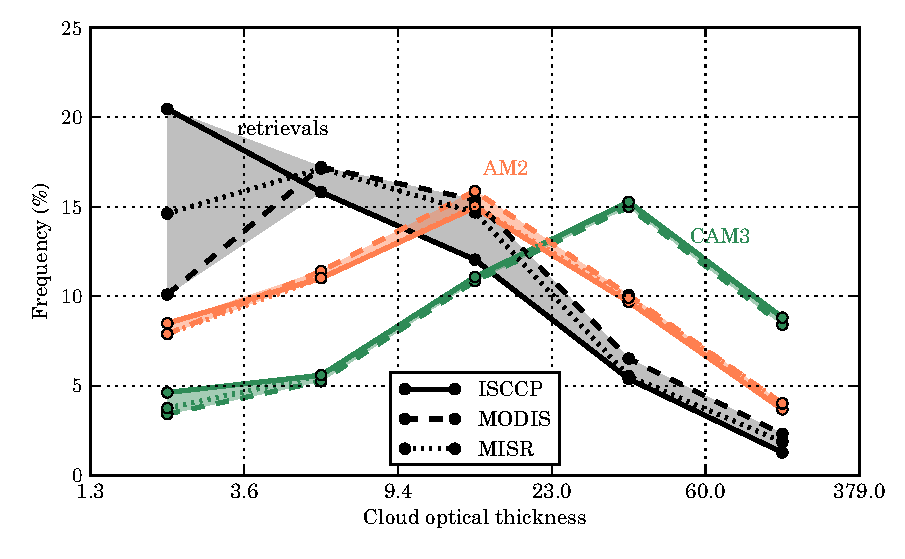
\includegraphics{../graphics/tau_cmip3amip.pdf}
    \caption{Global annual mean histogram of cloudiness with cloud optical thickness from ISCCP, MISR, and MODIS and the corresponding simulator diagnostics from CAM3 and AM2 AMIP simulations.}
    \label{tau_cmip3amip}
\end{figure}

\begin{figure}
    \centering
    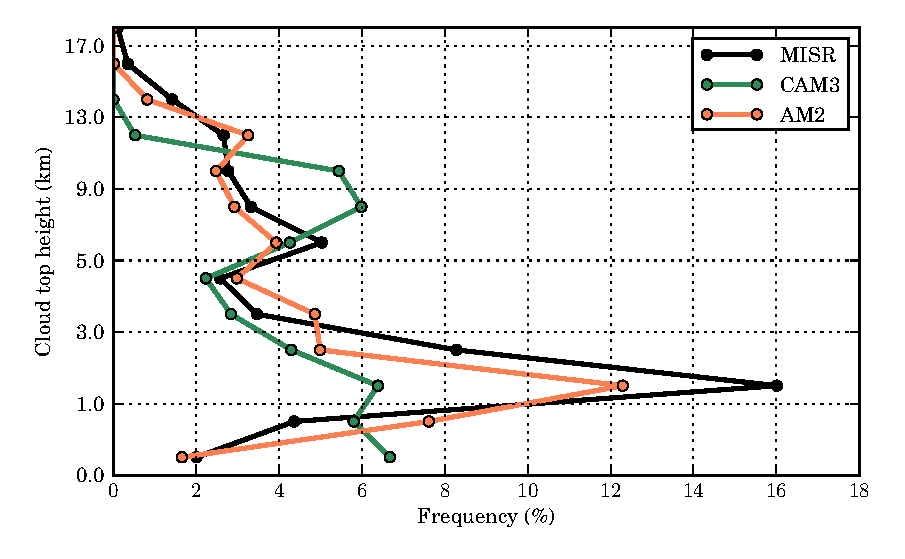
\includegraphics{../graphics/cth_cmip3amip.pdf}
    \caption{Global annual mean histogram of cloudiness with cloud top height from MISR and the MISR simulator diagnostic from CAM3 and AM2 AMIP simulations.}
    \label{cth_cmip3amip}
\end{figure}


CAM3 and AM2 differ in their simulation of high-topped cloud, with the CAM3 simulation overestimating and the AM2 simulation underestimating high-topped cloud amount. This is consistent with the biases in longwave cloud radiative effect: the overestimation of high-topped cloud in the CAM3 simulation causes an overestimation of the longwave heating effect of clouds, while the underestimation of high-topped cloud in the AM2 simulation causes an underestimation of the longwave heating effect of clouds.

Despite the wide range in space-time correlations and variance ratios amongst comparisons between observations from different instruments and their corresponding simulated model quantities, clouds in the AM2 simulation more closely match the observations by almost every statistical measure shown in Figure \ref{cldtypes_cmip3amip_taylor}. Exceptions to this are the comparison of ISCCP and ISCCP-simulated low-topped cloud, and the comparison of MISR and MISR-simulated mid-topped cloud, for which the variance ratios are closer to unity in the CAM3 simulation, indicating variability that more closely matches observations. In both of these cases, however, the space-time correlation with observations is much better for clouds in the AM2 simulation.

\subsection{Cloudiness in the tropics and subtropics}
The tropics are characterized by large-scale overturning circulations. These circulations give rise to regions of deep convective anvil-forming clouds associated with rising motion, and regions of shallow boundary layer cumulus or stratocumulus associated with large-scale subsidence. Different techniques have been employed to sample the different regimes in the tropics, including sub-setting by geographic region \citep[e.g.,][]{klein_and_hartmann_1993}, compositing by dynamical regime \citep[e.g.,][]{bony_et_al_2004,bony_and_dufresne_2005,medeiros_and_stevens_2009,medeiros_et_al_2011}, and sampling along a transect \citep[e.g.,][]{wyant_et_al_2010,bretherton_et_al_2010,teixeira_et_al_2011}. Each of these sampling strategies has their relative merits.

Sampling along a transect allows evaluation of the geographic distribution cloud types. Figure \ref{cldcth_cmip3amip_gpci} shows the frequency of occurrence of MISR cloud with cloud top height along the GEWEX Cloud System Study / Working Group on Numerical Experimentation (GCSS/WGNE) Pacific Cross-section Intercomparison (GPCI) Pacific Transect \citep{teixeira_et_al_2011} along with the corresponding MISR simulator diagnostic from CAM3 and AM2 AMIP simulations. The GPCI Pacific Transect \citep{teixeira_et_al_2011} consists of thirteen points from $(35^\circ~\text{N},125^\circ~\text{W})$ to $(1^\circ~\text{S},173^\circ~\text{W})$. This cross-section samples the range of cloud regimes found in the tropics and subtropics. The northeast endpoint falls in the heart of the persistent stratocumulus off the coast of California. Moving away from the coast along the transect, the stratocumulus decks break up and transition to shallow cumulus associated with the shallow convection of the trade winds. The cross-section continues further into the tropics, ending in the deep convection regime of the Inter-tropical Convergence Zone (ITCZ).

\begin{figure}
    \centering
    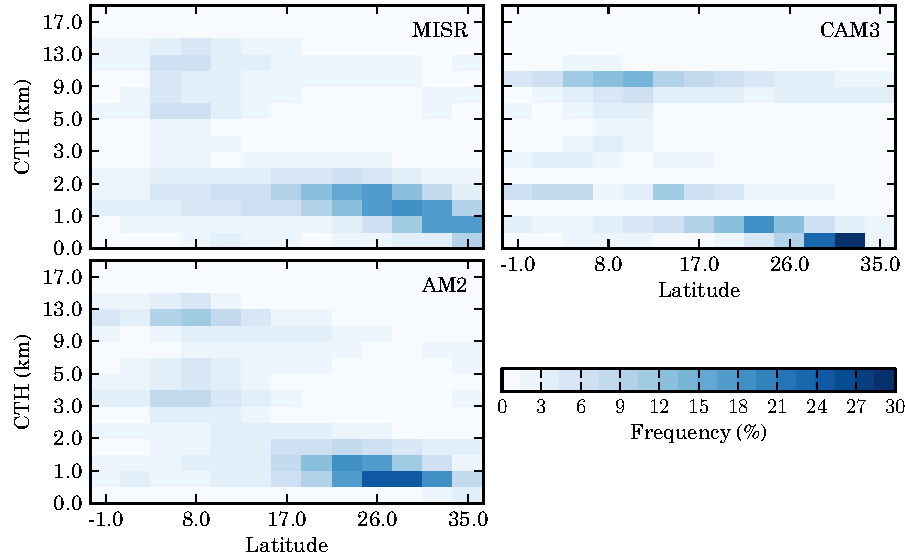
\includegraphics{../graphics/cldcth_cmip3amip_gpci.pdf}
    \caption[Histograms of summertime cloudiness with cloud top height along the GPCI Pacific transect from MISR and the MISR simulator diagnostic from CAM3 and AM2 AMIP simulations.]{Histograms of summertime (June, July, August) cloudiness with cloud top height along the GPCI Pacific transect from MISR and the MISR simulator diagnostic from CAM3 and AM2 AMIP simulations.}
    \label{cldcth_cmip3amip_gpci}
\end{figure}

The MISR observations show a large amount of low-topped (stratocumulus) cloud near the northeast endpoint of the cross-section (off the coast of California). Cloud top heights distinctly rise and cloud amounts decrease as the stratocumulus breaks up and transitions to broken trade cumulus in the shallow convection of the trade cumulus region. In the deep tropics, cloudiness equatorward of $10^\circ~\text{N}$ along the cross-section is characterized by high-topped cloud.

Both model simulations seem to at least broadly capture the three cloud regimes seen in the MISR observations. There is a large amount of low-topped cloud near the northeast endpoint of the cross-section in both model simulations, but the vertical distribution of cloud in this region differs from the observations. In both model simulations the cloud top heights are biased low in the atmosphere compared with the observations, and are clustered into only one or two cloud top height bins, whereas the distribution with cloud top height is more spread out in the observations. The low cloud top heights of cloud simulated by the models in this region are consistent with previous findings that have shown CAM3 to simulate boundary layers that are too shallow when compared with observations \citep{hannay_et_al_2009,medeiros_et_al_2011}. Figure \ref{hist2d_cmip3amip_california} shows the distribution of cloudiness in this region (defined in Table \ref{regions}) with cloud optical thickness and cloud top height. In addition to the low cloud top heights simulated by the models, total cloudiness and especially low-topped cloud is largely underestimated in this region. This is largely due to an underestimation of low-topped optically thin cloud, which is almost non-existent in the CAM3 simulation but accounts for a large amount of the cloudiness in the observations. The CAM3 simulation also biases low-topped cloud toward higher optical thickness values. The AM2 simulation has a distribution of low-topped cloud with optical thickness that more closely matches the observations, but with reduced magnitude. The underestimation of low-topped cloud in this region explains the underestimation of the shortwave cooling effect of clouds seen in Figure \ref{swcrebiases_cmip3amip_map}. Similar biases are present in simulation of cloudiness in the southeast Pacific stratocumulus as well (not shown).

\begin{table}
    \centering
    \begin{tabular}{lrrrr}
  \hline
  Region Name              & Lat South & Lat North & Lon West & Lon East \\ \hline
  California stratocumulus &  15 &  35 & 220 & 250 \\
  Hawaiian trade cumulus   &  15 &  35 & 150 & 210 \\
  Tropical western Pacific & -10 &  10 & 130 & 190 \\
% Southern Ocean           & -60 & -40 &   0 & 360 \\ \hline
  \hline
\end{tabular}

    \caption{Definition of region domains.}
    \label{regions}
\end{table}

\begin{figure}
    \centering
    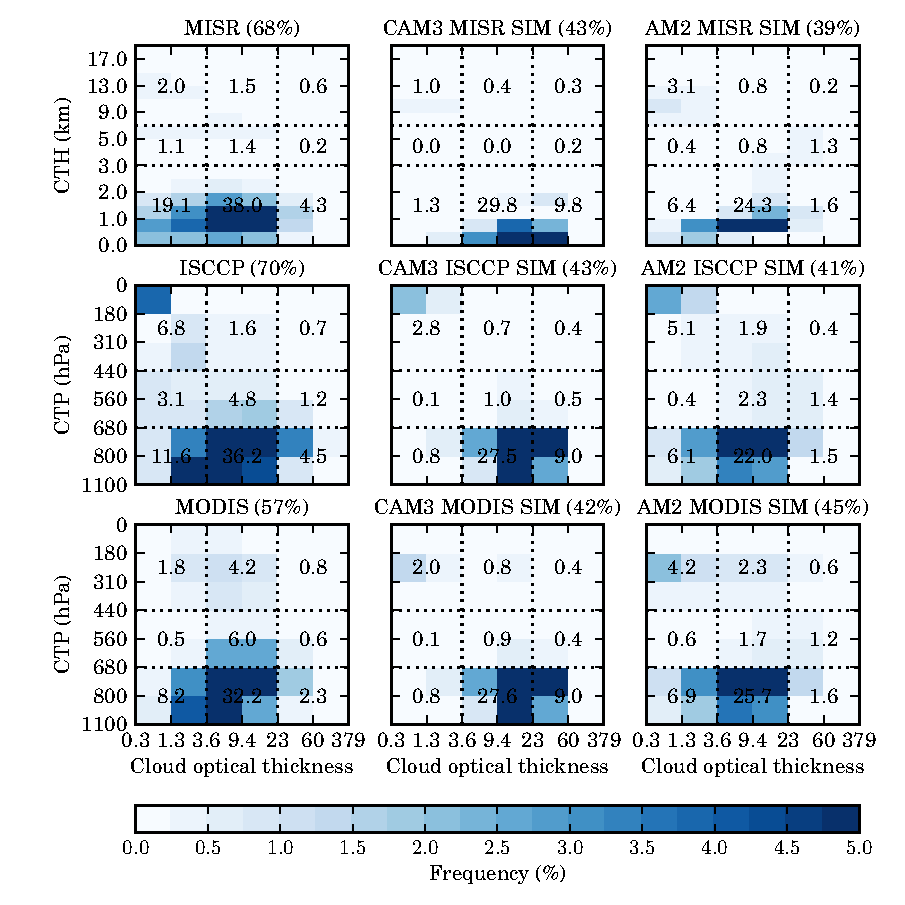
\includegraphics{../graphics/hist2d_cmip3amip_california.pdf}
    \caption[California stratocumulus joint histogram of summertime cloudiness with cloud optical thickness and cloud top height from MISR, ISCCP, and MODIS and the corresponding simulator diagnostics from CAM3 and AM2 AMIP simulations.]{California stratocumulus (Table \ref{regions}) joint histogram of summertime (June, July, August) cloudiness with cloud optical thickness and cloud top height (or pressure) from MISR, ISCCP, and MODIS and the corresponding simulator diagnostics from CAM3 and AM2 AMIP simulations.}
    \label{hist2d_cmip3amip_california}
\end{figure}

Figure \ref{cldcth_cmip3amip_gpci} shows a hint of an increase in cloud top heights from the stratocumulus (around $30^{\circ}$ N) into the cumulus transition (around $17^{\circ}$ N) in the CAM3 simulation, but in general both model simulations fail to capture the rising cloud top heights seen in the observations. In fact, CAM3 seems to almost entirely miss this important transition, instead rather abruptly jumping to the deep convective regime in the deep tropics. The transition in the AM2 simulation is somewhat abrupt as well. The misrepresentation of low-topped cloud in this region is particularly troubling in light of studies such as \cite{bony_and_dufresne_2005} that highlight the importance of boundary layer clouds in regions of large-scale subsidence. Figure \ref{hist2d_cmip3amip_hawaiian} shows the distribution of cloudiness with cloud optical thickness and cloud top height for the Hawaiian trade cumulus region (defined in Table \ref{regions}), which should contain large amounts of shallow trade cumulus. The MISR observations show that cloudiness in this region is dominated by low-topped optically thin cloud, consistent with trade cumulus. The model simulations, on the other hand, miss the majority of this cloud type, showing instead higher amounts of high-topped cloud more characteristic of the deep tropics (Figure \ref{hist2d_cmip3amip_twp}). The low-topped cloud that is present is biased toward higher optical thickness bins than seen in the observations. This pattern extends throughout the mid-topped cloud layers as well in both model simulations. High-topped cloud is generally over-estimated. The distribution of high-topped cloud with optical thickness in the AM2 simulation more closely matches observations, while the CAM3 simulation substantially overestimates high-topped optically thick cloud. The overestimation of high-topped cloud in this region in both models explains both the overestimation of shortwave cooling and longwave heating in this region.
\begin{figure}
    \centering
    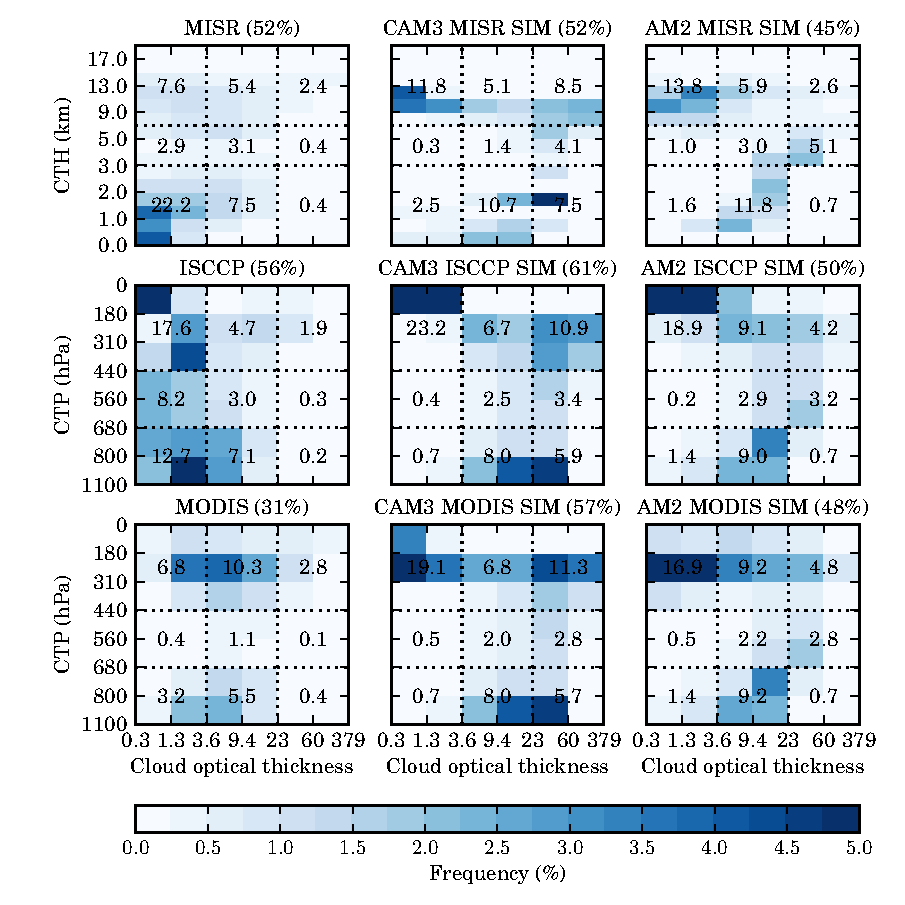
\includegraphics{../graphics/hist2d_cmip3amip_hawaiian.pdf}
    \caption[Hawaiian trade cumulus joint histogram of summertime cloudiness with cloud optical thickness and cloud top height from MISR, ISCCP, and MODIS and the corresponding simulator diagnostics from CAM3 and AM2 AMIP simulations.]{California stratocumulus (Table \ref{regions}) joint histogram of summertime (June, July, August) cloudiness with cloud optical thickness and cloud top height (or pressure) from MISR, ISCCP, and MODIS and the corresponding simulator diagnostics from CAM3 and AM2 AMIP simulations.}
    \label{hist2d_cmip3amip_hawaiian}
\end{figure}

High-topped cloud in the deep tropics is overestimated in both CAM3 and AM2 simulations, although total cloudiness is underestimated by both models in this region (except compared to MODIS, but note that this is the MODIS \emph{retrieval} cloud amount, which represents a substantially lower population of pixels due to clear-sky restoral). The overestimation of high-topped cloud is apparent in Figure \ref{cldcth_cmip3amip_gpci}, but is more clearly demonstrated by Figure \ref{hist2d_cmip3amip_twp}, which shows the distribution of cloudiness with cloud optical thickness and cloud top height in the tropical western Pacific region (defined in Table \ref{regions}). The underestimation of total cloudiness in this region is due to the fact that low-topped cloud seems to almost disappear in the model simulations, although this may be partly accounted for by the overestimation of high-topped cloud here. Recall that the purpose of the MISR simulator is to simulate the properties that MISR would retrieve in the model-generated world. An excess of high-topped clouds would prevent MISR from seeing any underlying low-topped clouds, and so an overestimation of MISR-simulated high-topped clouds would be expected to be accompanied by an underestimation of low-topped clouds. As noted in the Hawaiian trade cumulus region, cloudiness throughout the low and mid-level bins is biased toward higher optical thickness in both model simulations.

The MISR observations show a layer of relatively high cloud amount associated with the tropical freezing level in the $5$ to $7$ km cloud top height bin \citep{johnson_et_al_1999}, apparent in Figure \ref{cldcth_cmip3amip_gpci}. The CAM3 simulation completely misses this cloud layer. \cite{marchand_and_ackerman_2010} found that simulations from the Multi-scale Modeling Framework (MMF) model (which replaces the cloud parameterizations in CAM with a 2-dimensional cloud resolving model) also fail to simulate this freezing level cloud layer. Interestingly, the AM2 simulation does show a layer of cloud in the mid-troposphere, although this layer appears too low in the atmosphere (between $3$ and $4$ km) to be associated with the tropical freezing level.
\begin{figure}
    \centering
    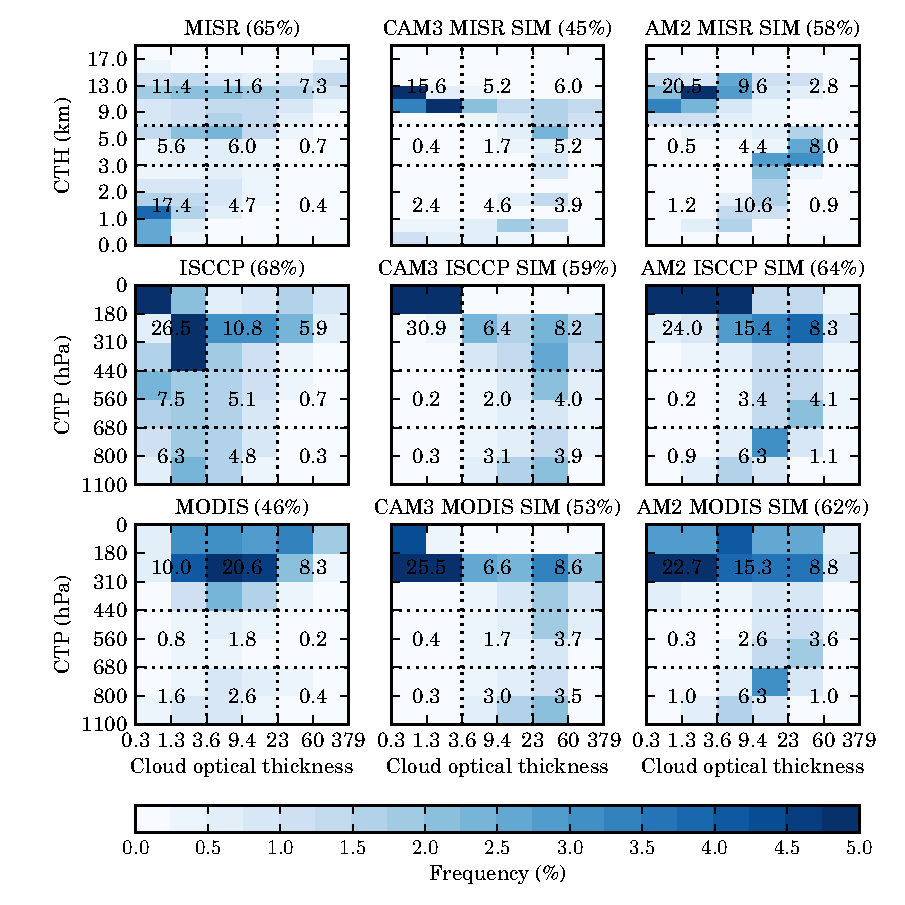
\includegraphics{../graphics/hist2d_cmip3amip_twp.pdf}
    \caption[Tropical western Pacific joint histogram of summertime cloudiness with cloud optical thickness and cloud top height from MISR, ISCCP, and MODIS and the corresponding simulator diagnostics from CAM3 and AM2 AMIP simulations.]{California stratocumulus (Table \ref{regions}) joint histogram of summertime (June, July, August) cloudiness with cloud optical thickness and cloud top height (or pressure) from MISR, ISCCP, and MODIS and the corresponding simulator diagnostics from CAM3 and AM2 AMIP simulations.}
    \label{hist2d_cmip3amip_twp}
\end{figure}

\section{Discussion}
The implementation of COSP in climate models allows for their robust evaluation of cloudiness by comparison with multiple independent satellite remote sensing datasets. The use of output from MISR and MODIS simulators in addition to the ISCCP simulator increases confidence in findings from previous evaluation studies using only the ISCCP simulator. 

CAM3 and AM2 have been shown to exhibit large biases in the simulation of present day clouds in this study, both in the geographic distribution of cloudiness and in the distribution of cloudiness with cloud top height and optical thickness. The fact that each model reasonably simulates top of atmosphere radiative fluxes is likely due in large part to compensation of the radiative effect of these different biases identified.

Total cloudiness has been demonstrated to be underestimated in both CAM3 and AM2 AMIP simulations when compared with observations from ISCCP, MISR, and MODIS in the global annual mean over the entire record of each dataset. This is primarily due to underestimation of low-topped cloud in both of these models. The underestimation of low-topped cloud is consistent with \cite{zhang_et_al_2005}, who also found mid-topped cloud to be underestimated by all models in their intercomparison when compared with ISCCP observations. In this study, however, mid-topped cloud was not found to be underestimated by AM2 when comparisons with MISR and MODIS observations and simulators were included, emphasizing the value in including multiple independent observations in model intercomparisons.

Total cloudiness has also been demonstrated to be underestimated in many of the regions considered here, despite differences in the sign of regional biases in shortwave and longwave cloud radiative effect. This points to compensating biases in the cloud radiative properties. Although total and especially low-topped cloud is underestimated in both CAM3 and AM2 AMIP simulations, both models are shown here to bias the distribution of cloudiness with cloud optical thickness toward higher optical thickness, due to an underestimation of optically thin cloud and optically intermediate cloud an overestimation optically thick cloud. This is a well known model bias identified by \cite{zhang_et_al_2005} using ISCCP observations and the ISCCP simulator implemented in ten different climate models, which included the NCAR CAM (version 2, an earlier version than used in this study) and the GFDL AM (version 2). The inclusion of comparisons using MISR and MODIS observations and simulators increases confidence in this finding.

The underestimation of total cloudiness and the overestimation of the optical thickness of clouds demonstrates compensating biases on the top of atmosphere radiative fluxes in these models. The presence of compensating errors in the cloud radiative properties simulated by climate models has been suggested by others \citep[e.g., ][]{webb_et_al_2001,weare_2004,zhang_et_al_2005}.

The magnitude of the shortwave cloud radiative effect is shown to be underestimated in regions known to be characterized by persistent stratocumulus. This is a common problem in climate models, and was recognized specifically for the California stratocumulus in other models by \cite{webb_et_al_2001}. In that study, they note that the underestimation of the magnitude of the shortwave cloud radiative effect in this region is due mainly to an underestimation of cloudiness in this region. The underestimation of cloudiness in stratocumulus regions is a bias common in both climate models and re-analyses \citep{duynkerke_and_teixeira_2001,bretherton_et_al_2004,siebesma_et_al_2004,stevens_et_al_2007}, and is demonstrated in this study for CAM3 and AM2 simulations.

\cite{webb_et_al_2001} also found cloud top heights that are lower than those retrieved by ISCCP in the California stratocumulus region. They cite that this could be caused by problems with the ISCCP retrieval of cloud top pressure, but here the addition of MODIS and especially MISR observations and simulators give compelling reason to believe that this is in fact a problem with the models. The low bias in cloud top heights is especially prevalent in the CAM3 AMIP simulation. This is likely due to simulation in models of boundary layers in the stratocumulus regions that are too shallow and poorly mixed compared with observations, as shown in numerous studies for both climate models and re-analyses \citep{bretherton_et_al_2004,siebesma_et_al_2004,stevens_et_al_2007,hannay_et_al_2009,medeiros_et_al_2011}

The shortwave cooling effect of clouds is overestimated in both CAM3 and AM2 AMIP simulations. \cite{webb_et_al_2001} found that other models show this same bias, and attributed overestimation of the shortwave cooling effect in this region to different factors in different models. In both CAM3 and AM2 simulations, the overestimation of shortwave cooling is caused by an overestimation of high-topped clouds and of the optical thickness of clouds in this region.

Subtropical boundary layer clouds in regions of large-scale subsidence are underestimated in CAM3 and AM2 due in large part to an underestimation of optically thin cloud in these regions. The transition from stratocumulus to shallow cumulus is also poorly represented. These cloud types have long been recognized as important in terms of the radiative energy budget \citep{randall_et_al_1984}. \cite{bony_and_dufresne_2005} point to boundary layer clouds in regions of large-scale subsidence as being the largest contributors to the spread in cloud feedbacks in the tropics. Poor simulation of these cloud types in present day climate simulations raises serious concerns about the ability of models to accurately represent tropical cloud feedbacks in a changing climate.

High-topped cloud is demonstrated to be overestimated in both models in the tropical western Pacific, although total cloudiness is again underestimated. This bias is not as well documented in the literature, but biases in the simulation of high-topped cloud could potentially affect the impact of low clouds on the radiative fluxes by the masking effect of high-topped clouds over low-topped clouds in cases of multi-layer cloud scenes. This masking of low clouds is demonstrated in this study in the tropical Pacific, where high-topped cloud is seen to be overestimated by both models while low-topped cloud is underestimated. Since passive sensor instrument simulators are used here, the deficit demonstrated is in \emph{instrument simulated} low-topped cloud, and may be due more to an overestimation of high-topped cloud over low cloud than to an underproduction of low cloud in the models. Although this exposes a limitation in comparisons made between models and passive remote sensing observations, it also highlights the importance of using instrument simulators in making comparisons between models and these types of observations. This example also illustrates another utility of the simulator strategy, in that comparisons are made between radiatively important clouds. In this example where high-topped cloud is overestimated in the models, regardless of any low-topped cloud beneath the high-topped cloud, the overestimation of high-topped cloud would act to increase the longwave heating effect of clouds. This is demonstrated in this study especially in the Hawaiian trade cumulus, and to a lesser extent in the tropical western Pacific. This result highlights the importance of accurate simulation of all cloud types in models.
